\chapter{Étude numérique}
	\minitoc
	\section{Utilisation du code \textsc{GADGET-2}}

		Le code que nous utilisons pour faire évoluer notre système est
		\textsc{Gadget-2}~\footnote{récupérable sur
		\url{http://www.mpa-garching.mpg.de/gadget/}}~\cite{gadget2},
		écrit par Volker \textsc{Springel}. Seule une petite partie de
		ce qu'il fait nous intéresse : nous n'allons utiliser que les
		options concernant le \og~tree code~\fg. Toutes les autres
		options ne concernent que les simulations cosmologiques ou
		pourraient induire un comportement du code qui nous ferait
		perdre de la précision sur les calculs.

		Pour fonctionner, \textsc{Gadget-2} a besoin d'un fichier de
		configuration, dans lequel nous devrons jouer sur certains
		paramètres, et d'un fichier de conditions initiales respectant
		un format précis.

		\subsection{Fichier de conditions initiales}

			Le fichier de conditions initiales doit avoir le format suivant :
			\begin{enumerate}
				\item un en-tête contenant le nombre de particule de chaque type (~Gaz, Halo, Disque, Bulbe, Étoiles, Bndry~),
				la masse pour chaque type, divers autres informations utiles essentiellement aux simulations cosmologiques,
				\item les positions de chaque particules,
				\item leurs vitesses,
				\item un identifiant permettant de repérer chaque particule.
			\end{enumerate}
			Chaque bloc devant être encadré par sa taille en mémoire.

		\subsection{Fichier de configuration}

			Dans ce fichier, nous n'allons jouer que sur certains paramètres :
			\begin{itemize}
				\item \verb|OmegaLambda| : paramètre cosmologique représentant la densité d'énergie du
					vide, en le mettant à 0, nous faisons savoir à \textsc{Gadget-2} que nous ne faisons pas
					de simulation cosmologique.
				\item \verb|UnitLength_in_cm|, \verb|UnitMass_in_g| et \verb|UnitVelocity_in_cm_per_s|
					sont les unités dans lesquelles sont données, respectivement, les positions, masses et vitesses des particules en
					centimètre, gramme en centimètre par seconde. Ce sont ces facteurs de conversion
					qui donne l'unité de temps interne à \textsc{Gadget-2}. Nous utilisons
					les parsecs ($ 1 pc = 3.086 \times 10^{18} cm$) pour les positions, les kilogrammes
					($1 kg = 1000 g$) pour la masse, et les mètres par seconde ($ 1 m.s^{-1} = 10^2 cm.s^{-1}$)
					pour les vitesses. Ces unités nous donnent comme unité de temps
					interne :
					\begin{align}
						v &= \frac{d}{t} \notag \\
						t &= \frac{d}{v} \notag \\
						t &= \frac{3.086 \times 10^{18}}{10^2} = 3.086 \times 10^{16} s \notag \\
						t &= 9.77894 \times 10^8 ans
					\end{align}
				\item \verb|SofteningStarsMaxPhys| : paramètre de lissage de la force, permettant d'éviter
					qu'elle \og~n'explose~\fg~à cause d'une collision entre 2 particules trop proches.
					C'est sur ce paramètre qu'il faut jouer pour assurer la stabilité du système sur
					un grand nombre de temps dynamiques.
				\item \verb|ErrTolTheta| : représente l'angle d'ouverture, ou résolution angulaire, minimum.
					Celui-ci est fixé à $0.5$ et n'est plus modifié ensuite.
			\end{itemize}

		\subsection{Lissage de la force}

			Nous souhaitons nous placer dans la limite fluide afin
			de minimiser les effets de relaxations dû aux
			collisions à deux corps. Pour cela, nous pouvons jouer
			sur deux paramètres : le nombre de particules que nous
			mettons dans le système, et le paramètre de lissage.
			Étant limité en temps, nous ne pouvons pas lancer de
			simulations avec un très grand nombre de corps : les
			plus grosses simulations que nous lançons ont 100 000
			particules, et occasionnellement 500 000. Pour une
			évolution pendant 100 temps dynamiques, elles prennent
			environ 709 minutes en les faisant tourner sur 8 cœurs,
			et cela peut aller jusqu'à 1020 minutes.

			Le lissage est une borne, en distance, en deçà de laquelle nous considérons un potentiel minimum valant :
			\begin{align}
				\psi(r_{i} \sim 0) = - G \dfrac{m_i}{r_{i} + \epsilon}
			\end{align}
			où $r_i$ est le module de distance d'une particule
			numérotée $i$. $\epsilon$ est le paramètre de lissage
			de la force. Afin de nous placer dans la limite fluide,
			$\epsilon$ doit être tel qu'il contienne un nombre
			$N_\epsilon$ de particule grand devant 1 mais petit
			devant le nombre total de particule du système.
			Habituellement, c'est $N_\epsilon$ qui est choisi,
			imposant ainsi $\epsilon$, mais nous avons choisi
			$\epsilon$ imposant ainsi $N_\epsilon$.

		%	Dans un amas, la densité est plus forte au centre que
		%	sur le bord. Les effets de relaxation sont donc plus
		%	important au centre, le $\epsilon$ doit y minimiser ces
		%	effets, même s'il n'a aucun effet sur les bords de
		%	l'amas.
			À cause d'instabilité, il est important de décrire la
			dynamique au centre de l'amas avec la meilleur
			précision possible. Il est donc nécessaire d'être dans
			la limite fluide au centre. Il est alors intéressant de
			le relier à la densité centrale, plutôt que d'utiliser
			une distance inter-particulaire moyenne. Nous
			définissons donc $\alpha$ tel que :
			\begin{align}
				\alpha = \dfrac{\rho(0)}{\rho_\mathrm{moy}} = \dfrac{\rho(0)}{M} \frac{4}{3} \pi R^3
			\end{align}
			avec $M$ la masse totale de l'amas, $R$ le rayon de
			l'amas, et $\rho(0)$ la densité centrale de l'amas. La
			densité d'un volume de taille $\epsilon$ et la densité
			de l'amas nous donne donc :
			\begin{align}
				\rho_\epsilon &= \alpha \rho_\mathrm{moy}					\notag \\
				N_\epsilon    &= \alpha \frac{4}{3} \pi \epsilon^3 \dfrac{3N}{4\pi R^3}	\notag \\
					      &= \alpha N \( \dfrac{\epsilon}{R} \)^{3}
			\end{align}
			$N$ étant le nombre total de particules de l'amas. $N$,
			$R$ et $\alpha$ étant fixés, nous sommes ainsi libres
			de choisir $N_\epsilon$ ou $\epsilon$ pour répondre à
			nos besoins.

	\section{Générateur de conditions initiales}

		Pour obtenir nos conditions initiales, qui devront suivre un
		profil de \textsc{King}, nous allons utiliser la méthode de
		réjection, l'une des plus facile à mettre en place. Nous allons
		tirer aléatoirement la position et la vitesse des particules
		dans une boîte, puis nous n'en garderons qu'une partie en
		utilisant la fonction de distribution comme densité de
		probabilité. Pour commencer, nous utilisons les limites de
		notre modèle pour restreindre nos tirages à une boîte de taille
		\mbox{$\left[ - r_{\mathrm{max}}; r_{\mathrm{max}} \right]$}
		pour les distances et \mbox{$\left[ -v_{\mathrm{max}};
		v_{\mathrm{max}}\right]$} pour les vitesses :

		\begin{itemize}
			\item vitesse maximum : l'énergie totale du système est bornée supérieurement par l'énergie de libération :
				\begin{align}
					E = \dfrac{1}{2} m v_i^2 + m\psi(r) &< E_l \notag \\
					E_l - m\psi(r) &> \dfrac{1}{2} m v_i^2 \notag \\
					v_\mathrm{max}^2 = 2\(\dfrac{E_l}{m} - \psi(r)\) &> v_i^2 \notag \\
					v_{\mathrm{max}} = \sqrt{2\(\dfrac{E_l}{m} - \psi(0)\)} > v_i &> - \sqrt{2\(\dfrac{E_l}{m} - \psi(0)\)} = - v_{\mathrm{max}}
				\end{align}
			\item distance maximum : cette distance est obtenue pour
				$m\psi(r_{\mathrm{max}}) = E_l$. Il nous faut donc connaître le potentiel.
		\end{itemize}

		Le potentiel n'ayant pas d'expression analytique, nous allons devoir réutiliser
		notre algorithme de résolution numérique utilisé dans les chapitres précédents pour
		modèliser un King.

		Il nous faut aussi pouvoir redimensionner les quantités obtenues. Pour cela, le
		programme récupère dans un fichier de configuration les dispersions de vitesse
		$\sigma_v^2$, rayon de c\oe ur $r_c$, temps de relaxation $T_c$ et distance au
		soleil $R_\odot$ dans les unités du catalogue de \textsc{Harris}. Toutes sont
		ensuite transformées en unités SI (~mètre, kilogramme, seconde~). Comme nous
		avons pu le voir dans le chapitre~\ref{King::Chapitre} traitant du modèle de
		King, la masse $m$ d'une particule n'influence pas le profil de densité final :
		\begin{align}
			r_c^2 &= \dfrac{\sigma^2}{4\pi G m \rho_0} \notag \\
			      &= \dfrac{(\sigma_v^2)^2 m}{8\pi G m \rho_0} \notag \\
			      &= \dfrac{(\sigma_v^2)^2}{8\pi G \rho_0} \notag \\
			\Rightarrow \rho_0 &= \dfrac{(\sigma_v^2)^2}{8\pi G r_c^2}
		\end{align}
		Pour redimensionner la densité, nous n'avons donc pas besoin de connaître la
		masse d'une particule. Ce constat nous permet de laisser ce paramètre libre et
		de jouer sur le nombre de particules dans le système. En effet, une fois la
		densité obtenue, nous pouvons l'intégrer sur le volume de l'amas pour trouver la
		masse totale de ce dernier, puis, connaissant le nombre de particules, en déduire
		la masse d'une étoile par la relation :
		\begin{align}
			m = \dfrac{M_{tot}}{\text{Nombre de particules}}
		\end{align}
		Déduire le reste des paramètres utiles pour le redimensionnement est ensuite
		assez simple.
		La distance maximum $r_{\mathrm{max}}$ est déduite de la résolution
		numérique des équations.

		Pour pourvoir tout redimensionner, nous avons aussi besoin de connaître l'énergie
		de libération de l'amas. Pour cela, nous utilisons le théorème de \textsc{Gauss}
		et un petit raisonnement simple. Par définition, nous avons :
		\begin{align}
			E_\mathrm{min} < E < E_l < 0 \ &\text{ et } \ E_l = \frac{p^2}{2 m} + m \psi(r)
			\intertext{soit :}
			\psi(r) = \frac{1}{m}\(E_l - \frac{p^2}{2 m}\)
			\intertext{La valeur maximale du potentiel est donc atteinte pour $p = 0$ :}
			\psi_\mathrm{max} = \psi(R) = \frac{E_l}{m}
			\intertext{Hors du système, le théorème de \textsc{Gauss} nous dit qu'il peut être vu comme une particule ponctuelle de masse $M$. Le potentiel hors de l'amas s'écrit donc :}
			\psi(r) = -\frac{G M}{r}
			\intertext{Par continuité, nous avons :}
			\psi(R) = \frac{E_l}{m} = -\frac{G M}{R}
		\end{align}

		Pour générer des nombres aléatoires dans l'intervalle voulu, nous utilisons la
		fonction \verb|double ran2(long seed)| tiré de~\cite{NumericalRecipesC}, dont
		nous nous servont ainsi :
		\lstset{language=C, label=algo::tirage, frame=shadowbox}
		\begin{lstlisting}
			double  x  = rmax - 2.0 * rmax * ran2(seed),
				y  = rmax - 2.0 * rmax * ran2(seed),
				z  = rmax - 2.0 * rmax * ran2(seed),
				vx = vmax - 2.0 * vmax * ran2(seed),
				vy = vmax - 2.0 * vmax * ran2(seed),
				vz = vmax - 2.0 * vmax * ran2(seed);
		\end{lstlisting}
		Notre système étant sphérique, nous ne devons pas avoir de vitesse et de module
		de distance supérieurs, respectivement, à $v_{\mathrm{max}}$ et
		$r_{\mathrm{max}}$, de plus nous avons une probabilité
		\mbox{$f(E)/f(E_\mathrm{min})$}
		d'avoir une particule d'énergie $E$. Cette énergie minimale est l'énergie
		potentielle d'une particule au centre de l'amas, et de vitesse nulle.
		Une fois qu'une particule respecte ces conditions et que \og les probabilités sont
		avec elle \fg, nous l'enregistrons.

		Le programme écrit au fur et à mesure les coordonnées cartésiennes et vitesses
		des particules selectionnées dans un fichier dans les unités standards : mètre
		pour les distances et mètre par seconde pour les vitesses.

	\section{Vérification des résultats\label{Verif_gene}} %du générateur}

		Maintenant que nous avons un générateur de conditions initiales, il convient de
		le vérifier. C'est-à-dire d'utiliser les coordonnées, vitesses et masses des
		particules pour remonter à des quantités comme la densité ou l'énergie de
		l'objet créé, puis de comparer ces quantités aux prédictions théoriques.
		Notamment, nous avons généré un profil de King, qui se doit donc d'être au
		Viriel, mais aussi d'avoir une certaine pente sur la densité, comme vu dans les
		précédents chapitres.

		Pour faire les vérifications, nous avons choisi d'utiliser des histogrammes.

		\subsection{Masse et densité}

			\begin{wrapfigure}{l}{0.28\textwidth}
				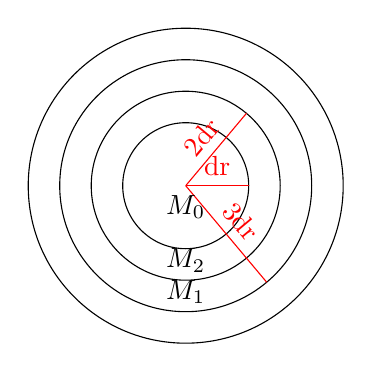
\begin{tikzpicture}[scale=0.8]
					\draw (2.5,2.5) circle(1);
					\draw (2.5,2.5) circle(1.5);
					\draw (2.5,2.5) circle(2);
					\draw (2.5,2.5) circle(2.5);
					\draw[red] (2.5,2.5) -- (3.5,2.5) node[midway, above] {$\mathrm{dr}$};
					\draw[red] (2.5,2.5) -- ++(50:1.5) node[sloped, above, midway] {$2 \mathrm{dr}$};
					\draw[red] (2.5,2.5) -- ++(-50:2) node[sloped, above, midway] {$3 \mathrm{dr}$};
					\draw (2.5,2.5) node[below]{$M_0$};
					\draw (2.5,1.15) node[below]{$M_1$};
					\draw (2.5,1.65) node[below]{$M_2$};
				\end{tikzpicture}
				\caption{Découpage de l'amas généré\label{schema::bin}}
			\end{wrapfigure}
			Le premier histogramme que nous générerons sera celui représentant
			la masse en fonction du rayon. Notre objet étant sphérique, nous allons le
			découper en intervalles de taille $\mathrm{dr}$ comme sur le schéma ci-contre. La fonction
			de masse représente la masse se trouvant dans l'intervalle \mbox{$\left[0; j \mathrm{dr}\right]$}.
			Pour la calculer, nous comptons le nombre de particules dans chaque chaque coquille sphérique de largeur $dr$ (~bin~), puis,
			après avoir multiplié par la masse d'un particule, nous sommons, pour le bin
			$j$, tous les bins inférieurs.

			En même temps que nous calculons la fonction de masse, nous pouvons calculer la
			densité en divisant la masse dans un bin par le volume du bin :
			\begin{align}
				\rho_\mathrm{bin} &= \dfrac{M_\mathrm{bin}}{V_\mathrm{bin}} \notag \\
				\rho_i = \rho\( (i+1) \mathrm{dr}\) &= \dfrac{M_{\mathrm{bin}\ i}}{V_{\mathrm{bin}\ i}} \\
					&= \dfrac{M_{\mathrm{bin}\ i}}{\frac{4}{3}\pi ( (i+1)\mathrm{dr})^3 - \frac{4}{3}\pi ( i\mathrm{dr})^3} \notag \\
					&= \dfrac{3 M_{\mathrm{bin}\ i}}{4 \pi \mathrm{dr}^3 \left[ (i+1)^3 - i^3\right]} \notag \\
					&= \dfrac{3 M_{\mathrm{bin}\ i}}{4 \pi \mathrm{dr}^3 \left[ 3 i^2 + 3 i + 1\right]} \\
					&= \dfrac{3 \(M_i - M_{i-1}\)}{4 \pi \mathrm{dr}^3 \left[ 3 i^2 + 3 i + 1\right]}
			\end{align}
			avec $M_{-1} = 0$.

			La densité obtenue et celle prévue par la résolution numérique sont très proche,
			comme le montre le graphique~\ref{Comp_gene-theo}.
			\begin{figure}[h!]
				\centering 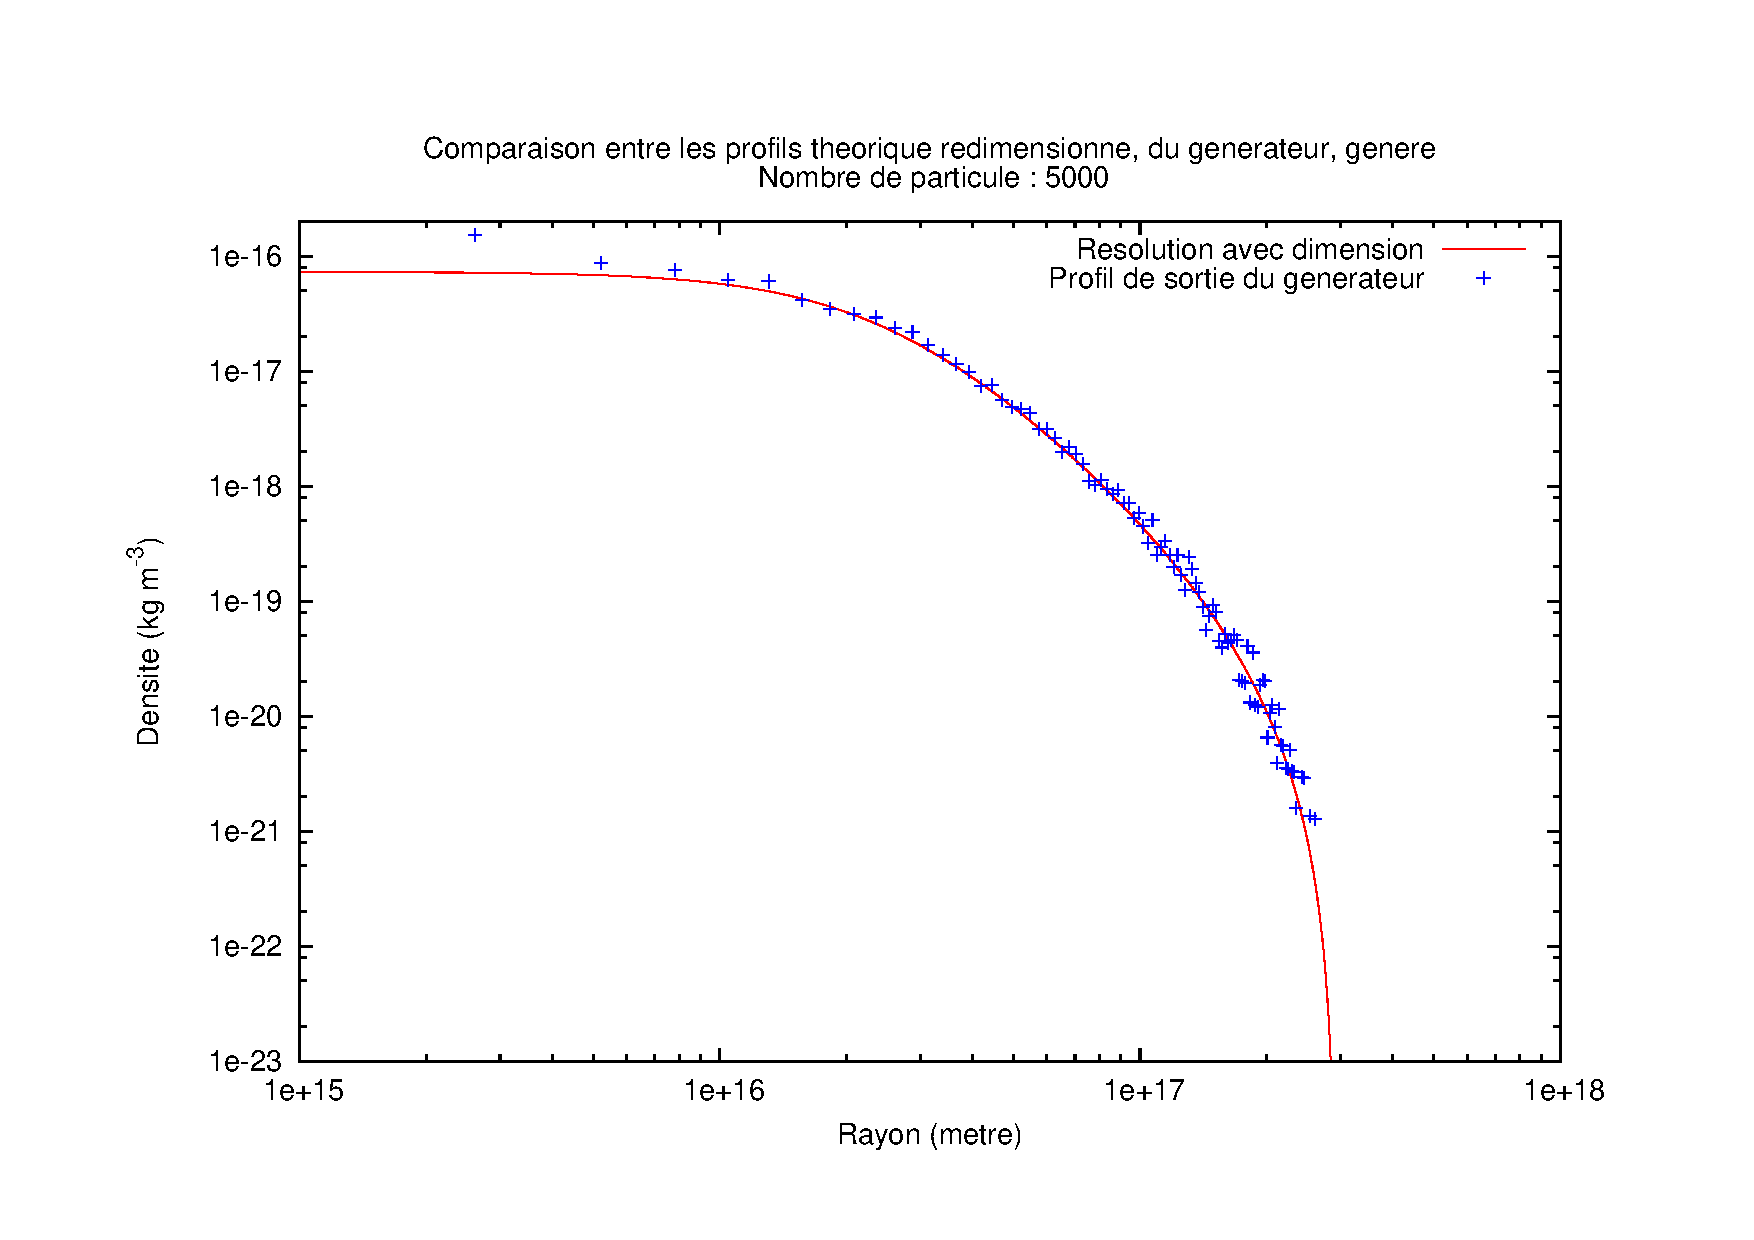
\includegraphics[scale=0.5]{graphe/Comp_dens_gene-theo_5000.pdf}
				\caption{Comparaison entre la résolution numérique et la densité donnée par le générateur\label{Comp_gene-theo}}
			\end{figure}

		\subsection{Énergie et potentiel}

			La partie la plus complexe de la vérification est le calcul de l'énergie. Deux
			choix s'offrent à nous :
			\begin{itemize}
				\item la méthode force brute : nous calculons l'énergie totale en utilisant
					l'expression newtonienne du potentiel :
					$$
						E_{tot} = \frac{1}{2}\sum_{i = 1}^{N} m_i v_i^2 - G \sum_{i = 1}^{N} \sum_{j < i} \dfrac{m_i m_j}{|| r_i - r_j ||}
					$$
					avec $N$ le nombre de particule Le problème de cette méthode est qu'elle nécessite $N^2$
				opérations et n'est donc pas intéressante lorsque nous travaillons avec un grand
				nombre de particules. De plus, si deux particules sont très proche,
				l'énergie potentielle va diverger.
				\item la réflexion : nous avons déjà calculé la densité, et nous avons
					la fonction de masse, nous avons tout ce qu'il nous faut pour
					avoir le potentiel à partir de l'équation de \textsc{Poisson}.
			\end{itemize}

			Nous allons calculer le potentiel en résolvant l'équation de \textsc{Poisson}. Voyons
			comment la résoudre avec ce que nous avons.
			\begin{align}
				\Delta\psi &= \frac{1}{r^2}\dfrac{d}{dr}\( r^2 \dfrac{d \psi(r)}{dr} \) = 4\pi G \rho(r) \notag \\
				r^2 \dfrac{d \psi(r)}{dr} &= 4\pi G \int_0^r \rho(r) r^2 dr = G M(r) \notag \\
				\intertext{La densité est une fonction continue par morceau, nous pouvons donc écrire :}
				M(r)    &= 4\pi \int_0^r \rho(r) r^2 dr \notag \\
					&= 4\pi \sum_{j = 0}^{i - 1} \int_{j \mathrm{dr}}^{(j+1)\mathrm{dr}} \rho_j r^2 dr + 4\pi \int_{r_{i-1}}^r r^2 dr \text{, $r\in\left[ r_{i - 1}; r_i \right]$} \notag \\
					&= 4\pi \sum_{j = 0}^{i - 1} \rho_j \left[ \dfrac{r^3}{3} \right|_{j \mathrm{dr}}^{(j+1)\mathrm{dr}} + 4\pi\rho_i\left[\dfrac{r^3}{3}\right|_{r_{i - 1}}^{r} \notag \\
					&= 4\pi \sum_{j = 0}^{i - 1} \dfrac{\rho_j}{3} \mathrm{dr}^3 \( (j+1)^3 - j^3)\) + \dfrac{4\pi \rho_i}{3} \(r^3 - i^3\mathrm{dr}^3\) \notag \\
					&= M(r_{i-1}) + \dfrac{4\pi \rho_i}{3} \(r^3 - i^3\mathrm{dr}^3\) \notag \\
				\intertext{Ceci nous permet alors d'écrire le potentiel :}
				\psi(r) - \psi(0) &= G \int_0^r \dfrac{M(r)}{r^2} dr \notag \\
				\psi\(r_i\) - \psi(0) &= G \sum_{j = 0}^{i} \left\{\int_{j \mathrm{dr}}^{(j+1)\mathrm{dr}} \dfrac{M(r_{j-1})}{r^2} + \dfrac{4\pi \rho_j}{3 r^2} \(r^3 - j^3\mathrm{dr}^3\) dr\right\} \notag \\
				\intertext{avec $ r_i = (i+1) \mathrm{dr} $}
				\psi(r_i) - \psi(0) &= G \sum_{j = 0}^{i} \left\{M_{j-1} \left[ \dfrac{-1}{r}\right|_{j \mathrm{dr}}^{(j+1)\mathrm{dr}} + \dfrac{4\pi \rho_j}{3} \( \left[ \dfrac{r^2}{2} \right|_{j \mathrm{dr}}^{(j+1)\mathrm{dr}} - j^3\mathrm{dr}^3 \left[ \dfrac{-1}{r}\right|_{j \mathrm{dr}}^{(j+1)\mathrm{dr}} \)\right\} \notag \\
						    &=  G \sum_{j = 0}^{i} \left\{\dfrac{1}{j ( j + 1 ) \mathrm{dr}} \( M_{j - 1} - \dfrac{4\pi \rho_j}{3}j^3\mathrm{dr}^3 \) + \dfrac{4\pi \rho_j}{6}\( 2 j + 1 \)\mathrm{dr}^2\right\}
				\intertext{Pour le bin central $j = 0$, nous avons :}
				\psi(dr) - \psi(0)  &=  G \dfrac{4\pi \rho_0}{6}\mathrm{dr}^2
			\end{align}

			Pour obtenir la constante $\psi(0)$, nous allons nous servir des conditions sur le bord du système. En effet, nous avons vu plus haut que :
			\begin{align}
				\psi_\mathrm{max} = \psi(R) &= - \frac{G M}{R} \\
				\intertext{Donc :}
				\psi(R) + \psi(0) - \psi(0) &= - \frac{G M}{R} \\
				\psi(0) &= - \frac{G M}{R} - \(\psi(R) - \psi(0)\) \\
				\psi(0) &= \frac{E_l}{m} - \(\psi(R) - \psi(0)\)
			\end{align}

			Le graphique~\ref{potentiel_5000} nous montre le potentiel théorique et le potentiel calculé par cette méthode.

			\begin{figure}[h!]
				\centering 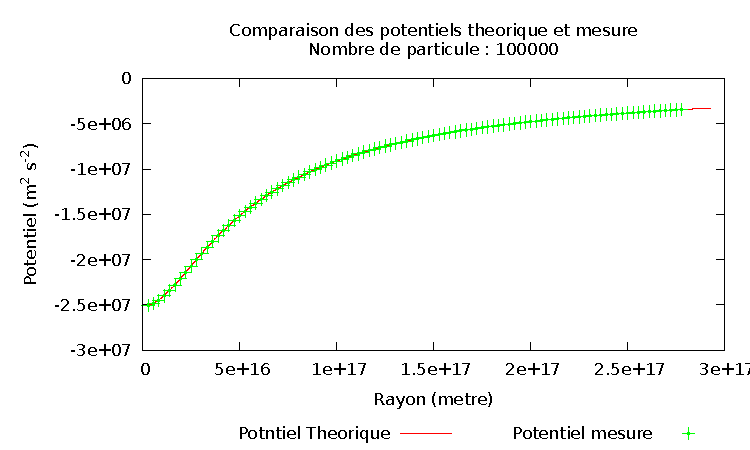
\includegraphics{graphe/Potentiel_ci-100000.pdf}
				\caption{Comparaison entre la résolution numérique et le potentiel donné par le générateur\label{potentiel_5000}}
			\end{figure}

		\subsection{Forme de l'amas}

			Maintenant que la densité et le potentiel de l'amas
			généré ont été vérifiés, il faut aussi vérifier que
			l'amas ne change pas de forme : nous générons un amas
			sphérique, nous devons~\footnote{il a en effet été
			montré qu'un \textsc{King} non collisionnel est
			stable~\cite{JPerez96}} conserver un amas sphérique
			après l'avoir fait évoluer. Pour vérifier que la forme
			de l'amas ne change pas, nous allons regarder comment
			évoluent les axes principaux d'inertie. Pour ce faire,
			nous allons calculer les valeurs propres de la matrice
			d'inertie :
			\begin{align}
				\mathfrak{I} &= \(\begin{array}{ccc}
							\int \(y^2 + z^2\) dm & - \int xy dm & - \int xz dm \\
							-\int xy dm & \int \(x^2 + z^2\) dm & - \int yz dm \\
							-\int xz dm & -\int yz dm & \int \(x^2 + y^2\) dm
						\end{array}\) \\
					     &= \(\begin{array}{ccc}
							A & - D & - E \\
							-D & B & - F \\
							-E & -F & C
						\end{array}\)\notag
				\intertext{L'équation aux valeurs propres va alors s'écrire :}
				\left|\mathfrak{I} - \lambda \mathbb{I}\right|  &= \(A - \lambda\)\left[\(B-\lambda\)\( C-\lambda\) - F^2\right] + D \(-D\(C-\lambda\) - F E\) - E \left[ D F + E\(B - \lambda\)\right] \notag %\\
			\end{align}
			polynôme d'ordre 3 que l'on résout avec la méthode de \textsc{Cardan}.

			Une fois ces valeurs propres obtenues, si elles
			existent, nous traçons l'évolution des rapports
			$\lambda_1 / \lambda_2$ et $\lambda_3 / \lambda_2$, les
			valeurs propres étant numérotées dans l'ordre
			décroissant \mbox{$\lambda_1 > \lambda_2 > \lambda_3$}.

	\section{Résultat des simulations}
		Les seules simulations que nous avons pu faire dans le cadre du stage sont des tests pour vérifier la stabilité de nos conditions initiales, ce qui représente déjà un travail important.

Nous avons donc commencé par générer des amas comportant un faible nombre de particules (~1000 ou 5000 particules~) afin de vérifier notre générateur, ce sont les résultats montrés par la courbe~\ref{Comp_gene-theo} pour 5000 particules, puis~\ref{potentiel_5000} pour 100000 particules.
Il nous faut maintenant vérifier que ces amas restent stables sur un grand nombre de temps dynamiques. Les simulations présentées dans cette section utilisent un amas réel dont les données ont été récupéré dans le catalogue de
\textsc{Harris} et à partir du travail fait dans les chapitres précédents. Il s'agit de l'amas NGC 288. Pour cet amas, les calculs analytiques donnent $\alpha = 439.72$.

Passons maintenant à l'étude de la stabilité sur le "long" terme de nos amas. Nous montrerons ici les résultats des tests
décrits dans la section~\ref{Verif_gene}.

Dans la table~\ref{eps_Neps}, nous avons indiqué quelles valeurs de $\epsilon$ nous avons utilisées : la valeur de $N_\epsilon$ correspondante, le nombre de particules qui sont au-delà du rayon des conditions initiales de l'objet,
et quelques autres informations utiles pour trouver la valeur qui nous intéresse.
	\begin{table}[h!]
		\begin{center}
			\begin{tabular}{|c|c|c|c|c|c|}
				\hline
				\multirow{2}{1cm}{$\epsilon\ \(pc\)$}	&	\multirow{2}{1cm}{$N_\epsilon$}	&	\multirow{2}{1cm}{$N_\mathrm{out}$}	&	\multirow{2}{3.5cm}{Fraction d'énergie cinétique emportée}	&	\multirow{2}{3.5cm}{Fraction d'énergie potentielle emportée}	&	\multirow{2}{2cm}{Courbes associées} \\
					&	&	&	&	&	\\
				\hline
				\hline
				$0.0194028$	&	$ 0.44 $		&	380	&	$ 0.00013573$			&	$ 0.00081092$	&	\ref{soft::0.019}, \ref{soft::0.019-Ax}\\
				\hline
				$0.05$		&	$ 7.52 $		&	239	&	$ 8.04628\times 10^{-5}$	&	$ 0.000488421$	&	\ref{soft::0.05}, \ref{soft::0.05-Ax}\\
				\hline
				$0.15$		&	$ 203.17 $		&	282	&	$ 9.91201\times 10^{-5}$	&	$ 0.00106241$	&	\ref{soft::0.15}, \ref{soft::0.15-Ax}\\
				\hline
				$0.20$		&	$ 481.58 $		&	653	&	$ 0.000265688$			&	$ 0.00265207$	&	\ref{soft::0.2}, \ref{soft::0.2-Ax}\\
				\hline
				$0.30$		&	$ 1625.34 $		&	919	&	$ 0.000433181$			&	$ 0.00466071$	&	\ref{soft::0.3}, \ref{soft::0.3-Ax}\\
				\hline
			\end{tabular}
		\end{center}
		\caption{Valeurs testés pour $\epsilon$ et $N_\epsilon$\label{eps_Neps}}
	\end{table}

	Discutons maintenant les résultats.

	\begin{description}
	%\paragraph{$\epsilon = 0.0194028$ :}
	\item[$\epsilon = 0.0194028$]
	Ce paramètre donne des résultats satisfaisants : sa densité évolue assez peu sur le temps de la simulation comparé aux valeur de $\epsilon > 0.05$, et ses axes d'inertie restent constant
	(~le bruit visible sur les graphes est dû au bruit statistique, bruit statistique dû au nombre fini de particules~). Par contre, le nombre de particules dans un volume de taille $\epsilon$ est trop petit : nous sommes trop loin de la limite fluide.

	%\paragraph{$\epsilon = 0.05$ :}
	\item[$\epsilon = 0.05$]
	Les fractions d'énergie potentielle et cinétique emportées par les particules sortantes sont minimum pour ce paramètre. De plus, sa densité et ses axes d'inertie évoluent peu, comme pour la valeur précédente.
	Cette fois, nous avons suffisamment de particules dans le volume de taille $\epsilon$.

\begin{figure}[h!]
	\centering 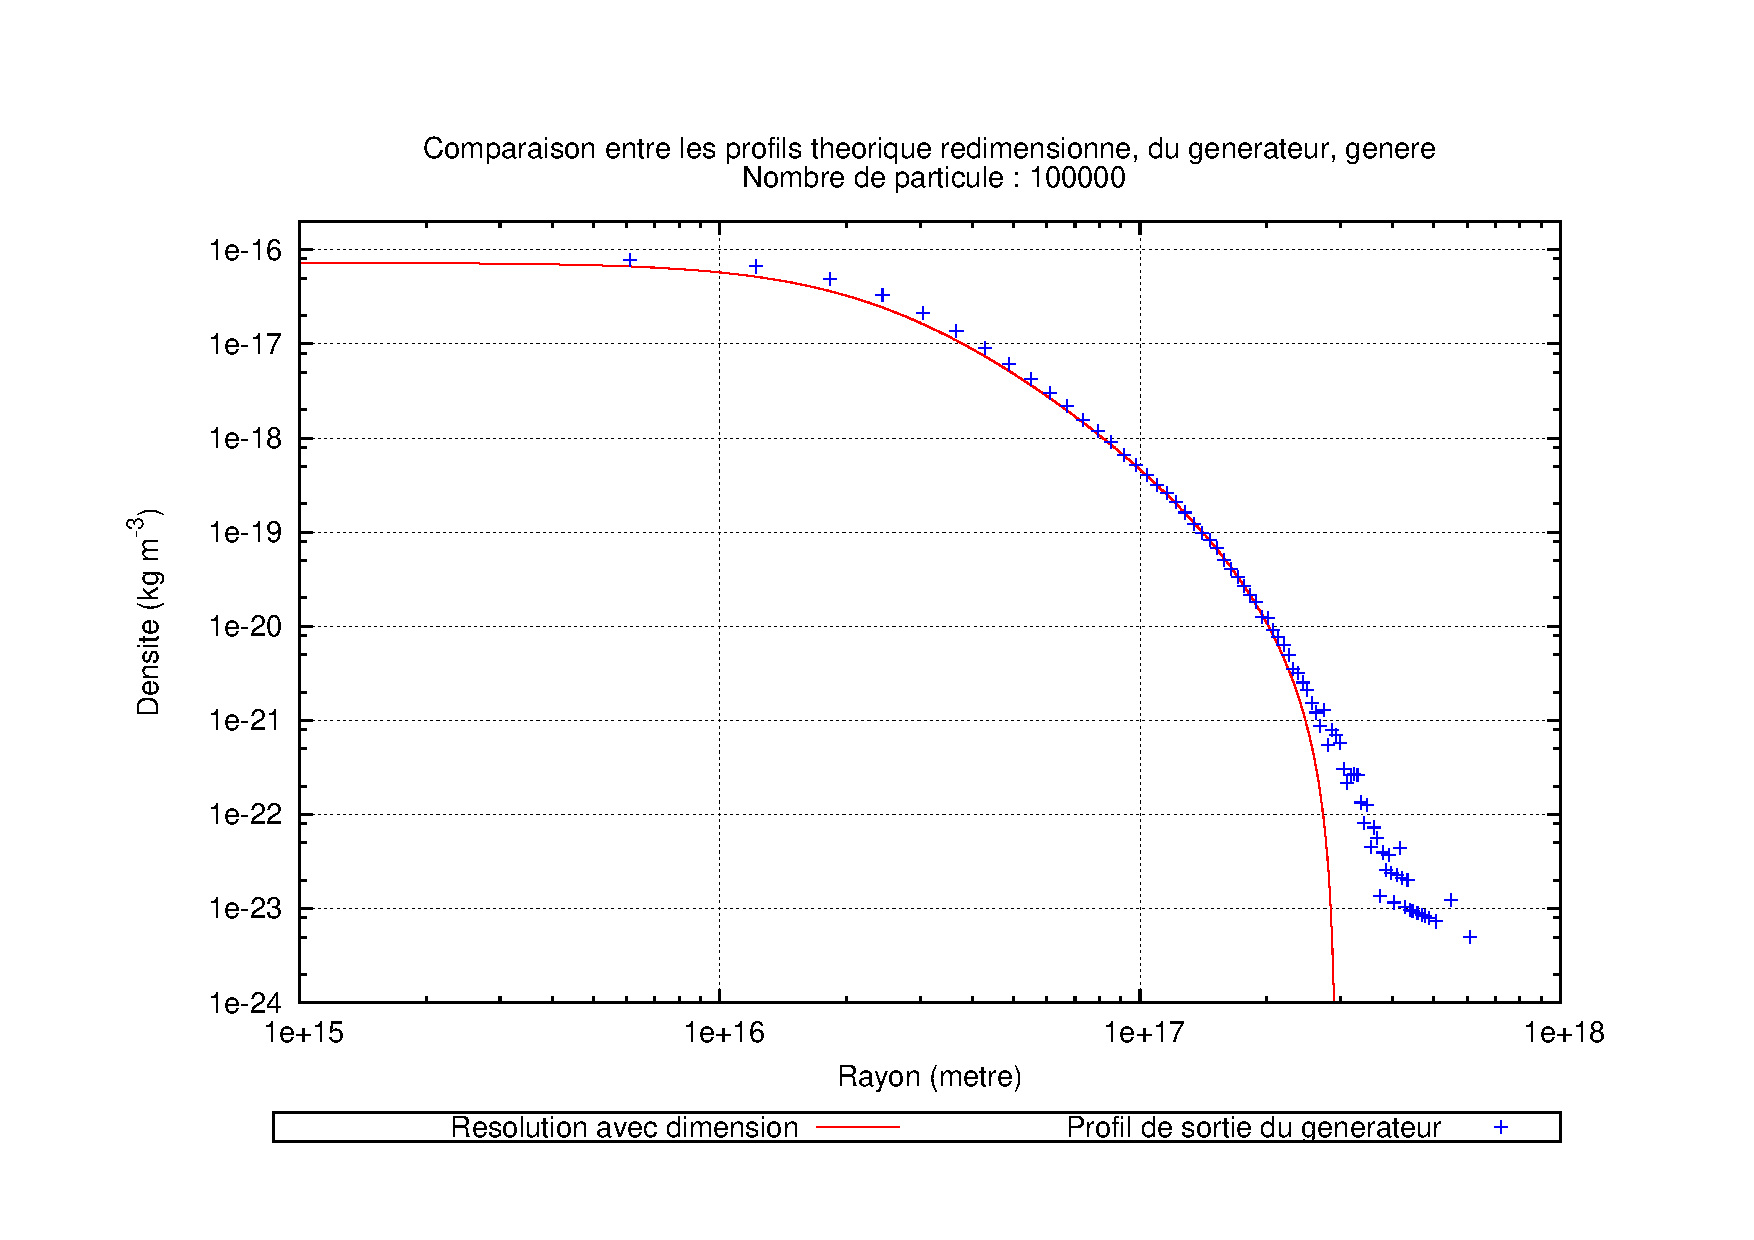
\includegraphics[scale=0.5]{graphe/Comp_dens_gene-theo_0-05.pdf}
	\caption{Comparaison entre la densité numérique et la densité après évolution : $\epsilon = 0.05$\label{soft::0.05}}
\end{figure}

\begin{figure}[h!]
	\centering 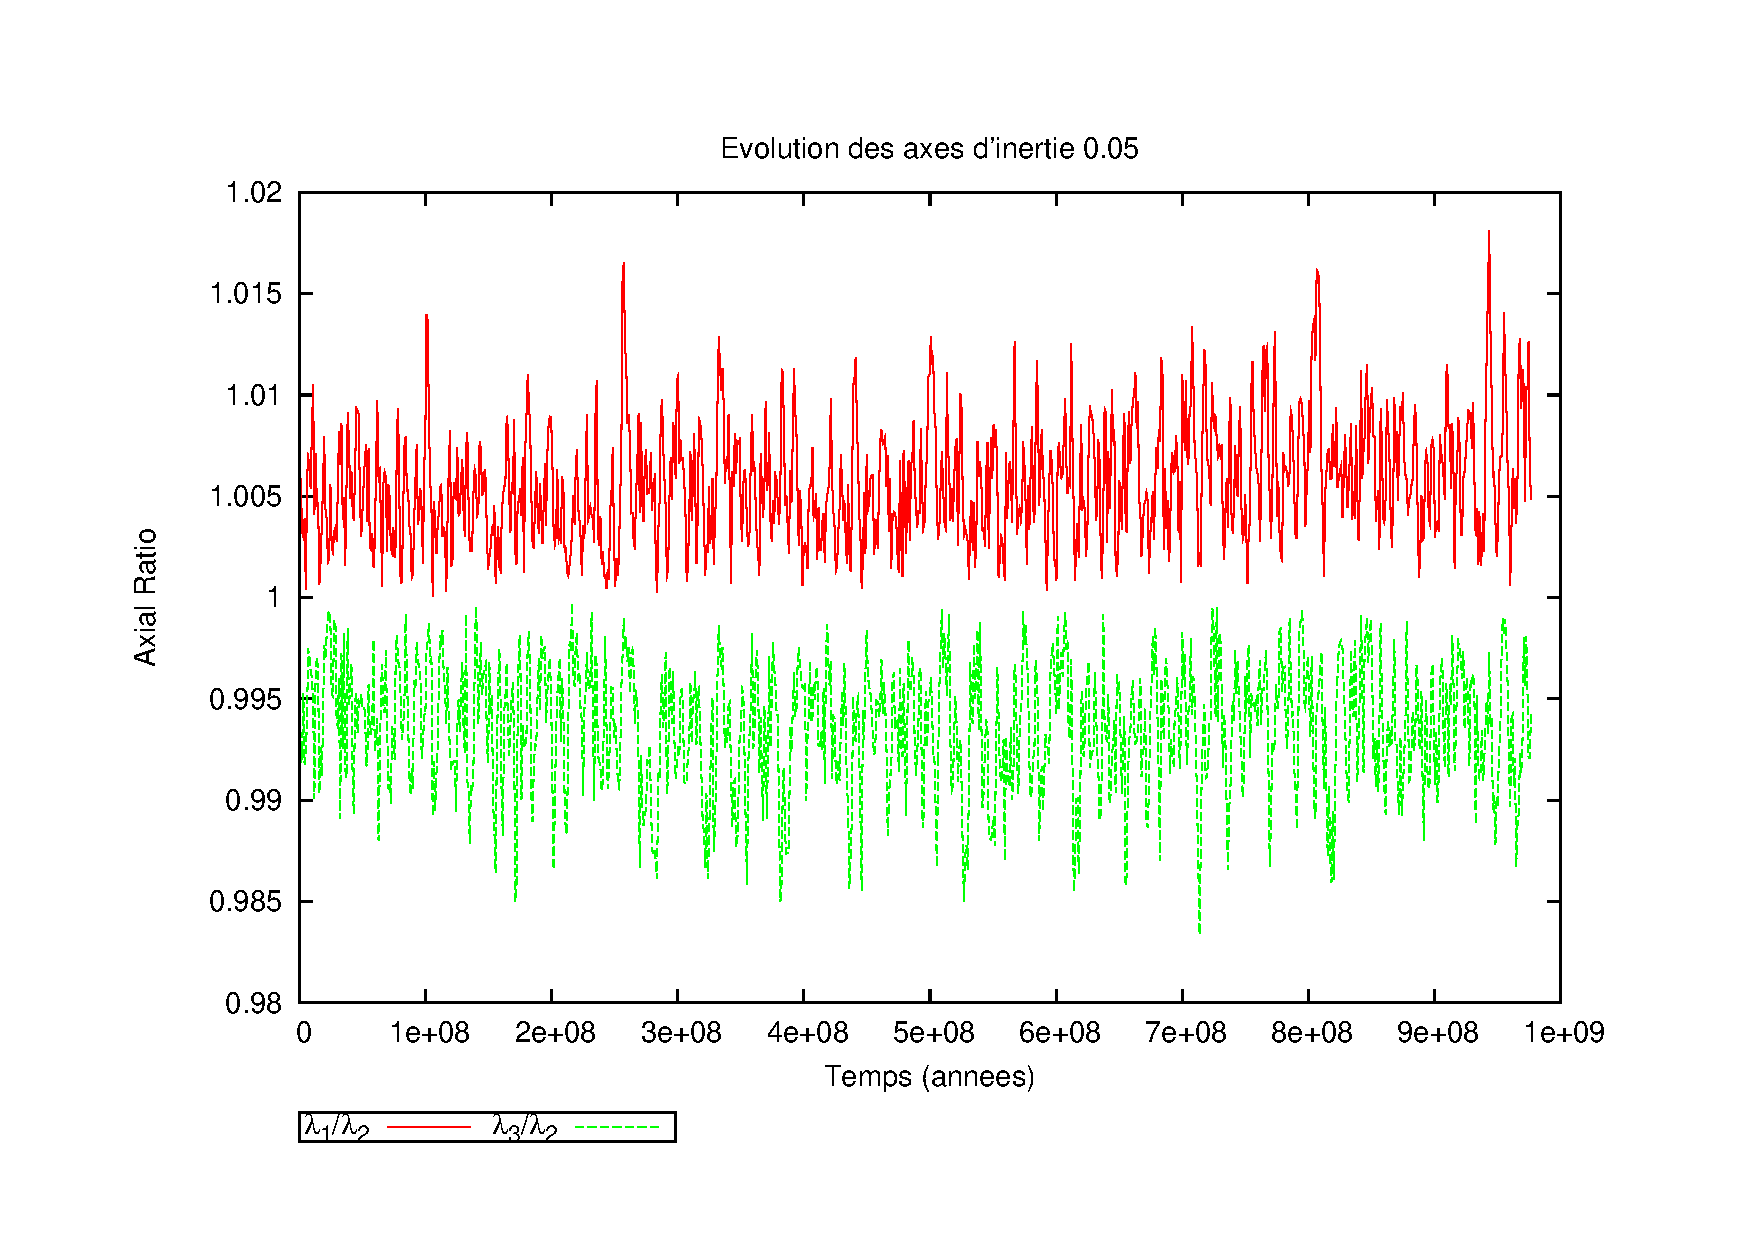
\includegraphics[scale=0.5]{graphe/Axial_ratio_0-05.pdf}
	\caption{Évolution des rapports des axes d'inertie : $\epsilon = 0.05$\label{soft::0.05-Ax}}
\end{figure}

	%\paragraph{$\epsilon = 0.15$ :}
	\item[$\epsilon = 0.15$]
	Pour ce paramètre, la fraction d'énergie potentielle emportée est de l'ordre de $0.1\%$, ce qui représente un changement important pour le rapport du Viriel $2 E_c/E_p$
	(~avec $E_c$ l'énergie cinétique et $E_p$ l'énergie potentielle~) : le profil de densité a complétement changé, l'amas s'est étendu.
	Par contre, il commence à se passer des choses intéressantes au niveau des axes d'inertie : pendant une grande partie de la simulation l'amas conserve sa forme, puis une instabilité arrive et il se déforme. % selon
%	l'un des axes, mais reste constant sur le second.
	\item[$\epsilon > 0.15$]
	Les valeurs supérieurs de $\epsilon$ ne sont alors clairement pas intéressante. De plus, ces valeurs sont trop proches du rayon de cœur de l'amas qui est de l'ordre de $10^{16}\ m = 0.32\ pc$ : en lissant toute
	la partie centrale de l'amas, nous changeons sa dynamique. En effet, il suffit de voir que, en augmentant le paramètre de lissage, l'instabilité menant à une déformation arrive de plus en plus tôt.
	Les déformations deviennent plus violentes.
	\end{description}

	La valeur de lissage optimale se trouve donc entre $\epsilon = 0.05$ et $\epsilon = 0.15$, pour une dizaine de particule (~pour $N_\epsilon = 10$, $\epsilon \sim 0.05497\ pc$~).




